\chapter{Configuración de OpenPGP en Thunderbird}

\section{Descripción del proceso}

Mozilla Thunderbird incorpora nativo para OpenPGP. Para poder firmar y cifrar correos con OpenPGP es necesario generar un par de claves personal y asociarlo a la cuenta de correo. El proceso se realiza desde la sección \textbf{Ajustes de cuenta $\rightarrow$ Cifrado de extremo a extremo}.

\section{Paso 1 -- Acceso a la sección de cifrado de extremo a extremo}

Accedemos a \textbf{Ajustes de cuenta} y seleccionamos \textbf{End-To-End Encryption} en el menú lateral. Thunderbird muestra que no existe ninguna clave OpenPGP asociada a la cuenta y ofrece el botón \textbf{Add Key\ldots} para iniciar el proceso.

\begin{figure}[H]
    \centering
    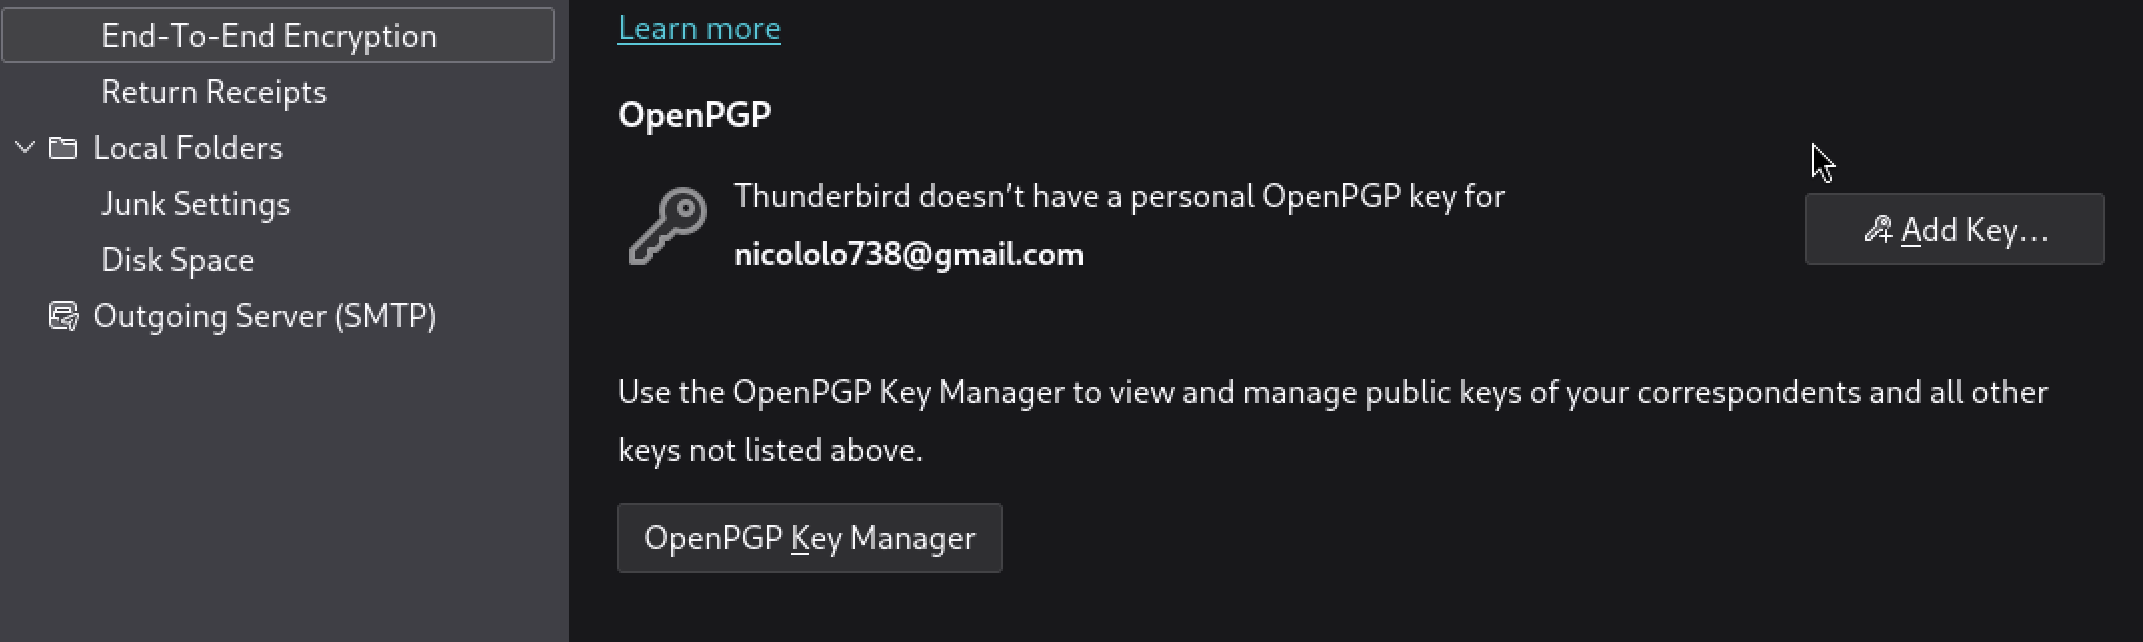
\includegraphics[width=\textwidth]{Imagenes/1-AccountSettingsEndToEndEncSect.png}
    \caption{Sección \textit{End-To-End Encryption} en los ajustes de cuenta de Thunderbird}
    \label{fig:e2e_section}
\end{figure}

\section{Paso 2 -- Selección del tipo de operación}

Al pulsar \textbf{Add Key\ldots}, Thunderbird presenta un diálogo con dos opciones:

\begin{itemize}[label=\textbullet]
    \item \textbf{Create a new OpenPGP Key}: genera un nuevo par de claves desde cero.
    \item \textbf{Import an existing OpenPGP Key}: importa un par de claves ya existente.
\end{itemize}

Dado que no disponemos de claves previas, seleccionamos \textbf{Create a new OpenPGP Key} y pulsamos \textit{Continue}.

\begin{figure}[H]
    \centering
    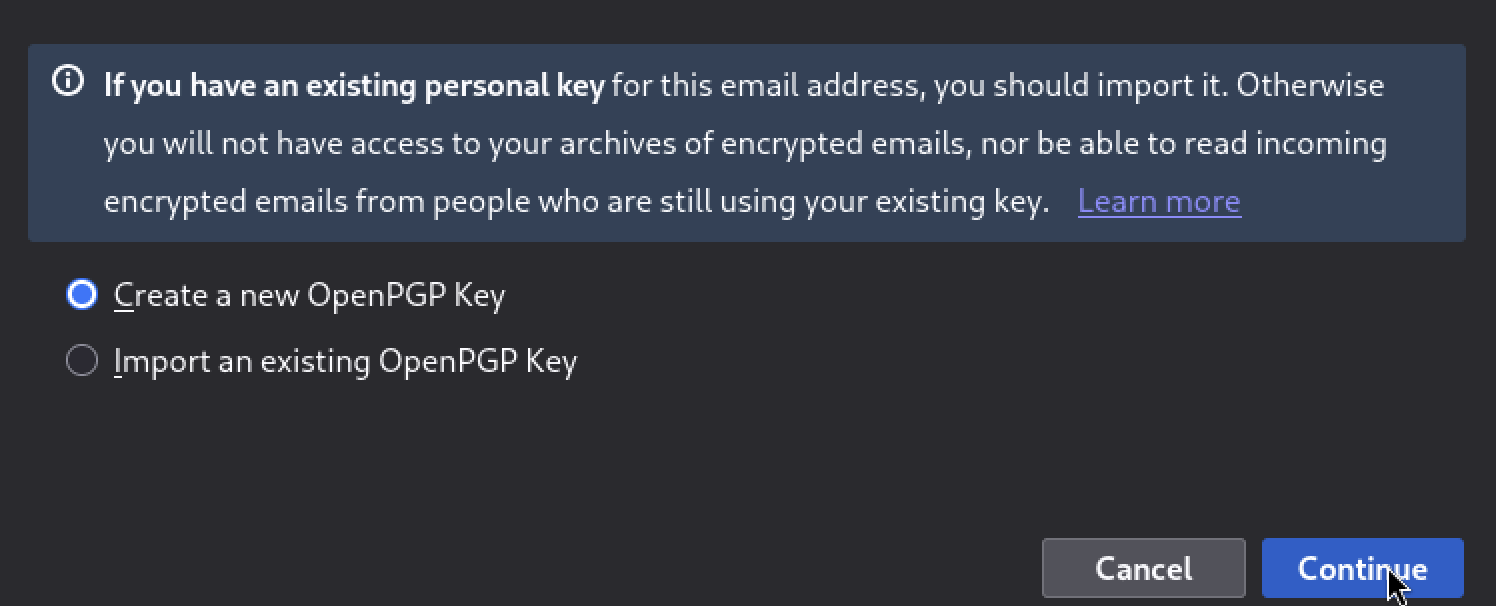
\includegraphics[width=0.85\textwidth]{Imagenes/2-CreationOfOpenPGPkey1.png}
    \caption{Diálogo de selección: crear o importar clave OpenPGP}
    \label{fig:seleccion_tipo_clave}
\end{figure}

\section{Paso 3 -- Configuración de la clave}

Se presenta el formulario \textbf{Generate OpenPGP Key} con los siguientes parámetros configurables:

\begin{itemize}[label=\textbullet]
    \item \textbf{Identity}: se asigna automáticamente a \texttt{Nicololo <nicololo738@gmail.com>}.
    \item \textbf{Key expiry}: se selecciona \textit{Key does not expire} para que no caduque.
    \item \textbf{Key type}: \textit{ECC (Elliptic Curve)} --- algoritmo moderno y eficiente.
    \item \textbf{Key size}: 256 bits o 384 bits dependiendo de la curva que utilice Thunderbird. Segun la documentación, ECC-256 es la que se selecciona por defecto pero hay soporte para P‑384, P‑521 y las curvas de EdDSA.
\end{itemize}

\begin{figure}[H]
    \centering
    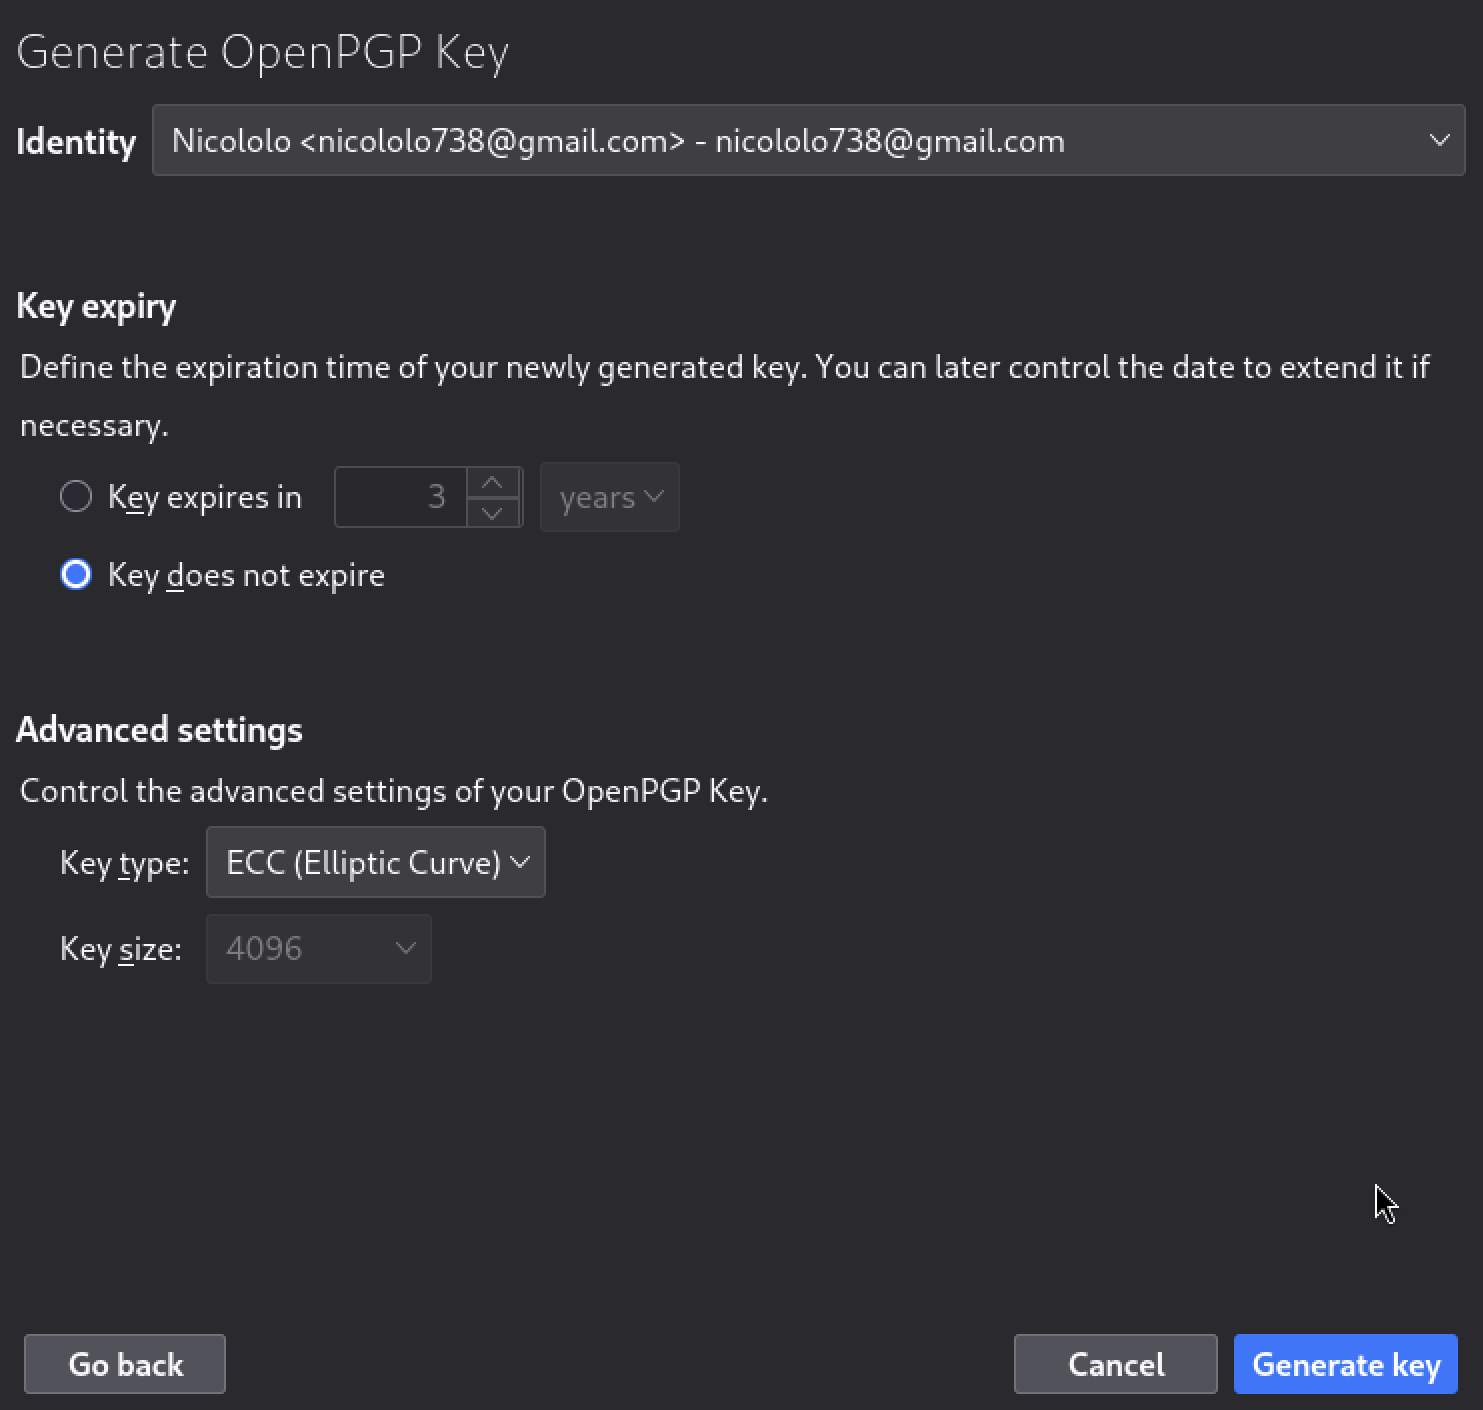
\includegraphics[width=0.85\textwidth]{Imagenes/3-CreationOfOpenPGPkey2.png}
    \caption{Formulario de configuración de la nueva clave OpenPGP (ECC, sin caducidad)}
    \label{fig:config_generacion_clave}
\end{figure}

\section{Paso 4 -- Confirmación y generación}

Tras pulsar \textbf{Generate key}, Thunderbird muestra un diálogo de confirmación advirtiendo que el proceso puede tardar varios minutos. Se pulsa \textbf{Confirm} para iniciar la generación.

\begin{figure}[H]
    \centering
    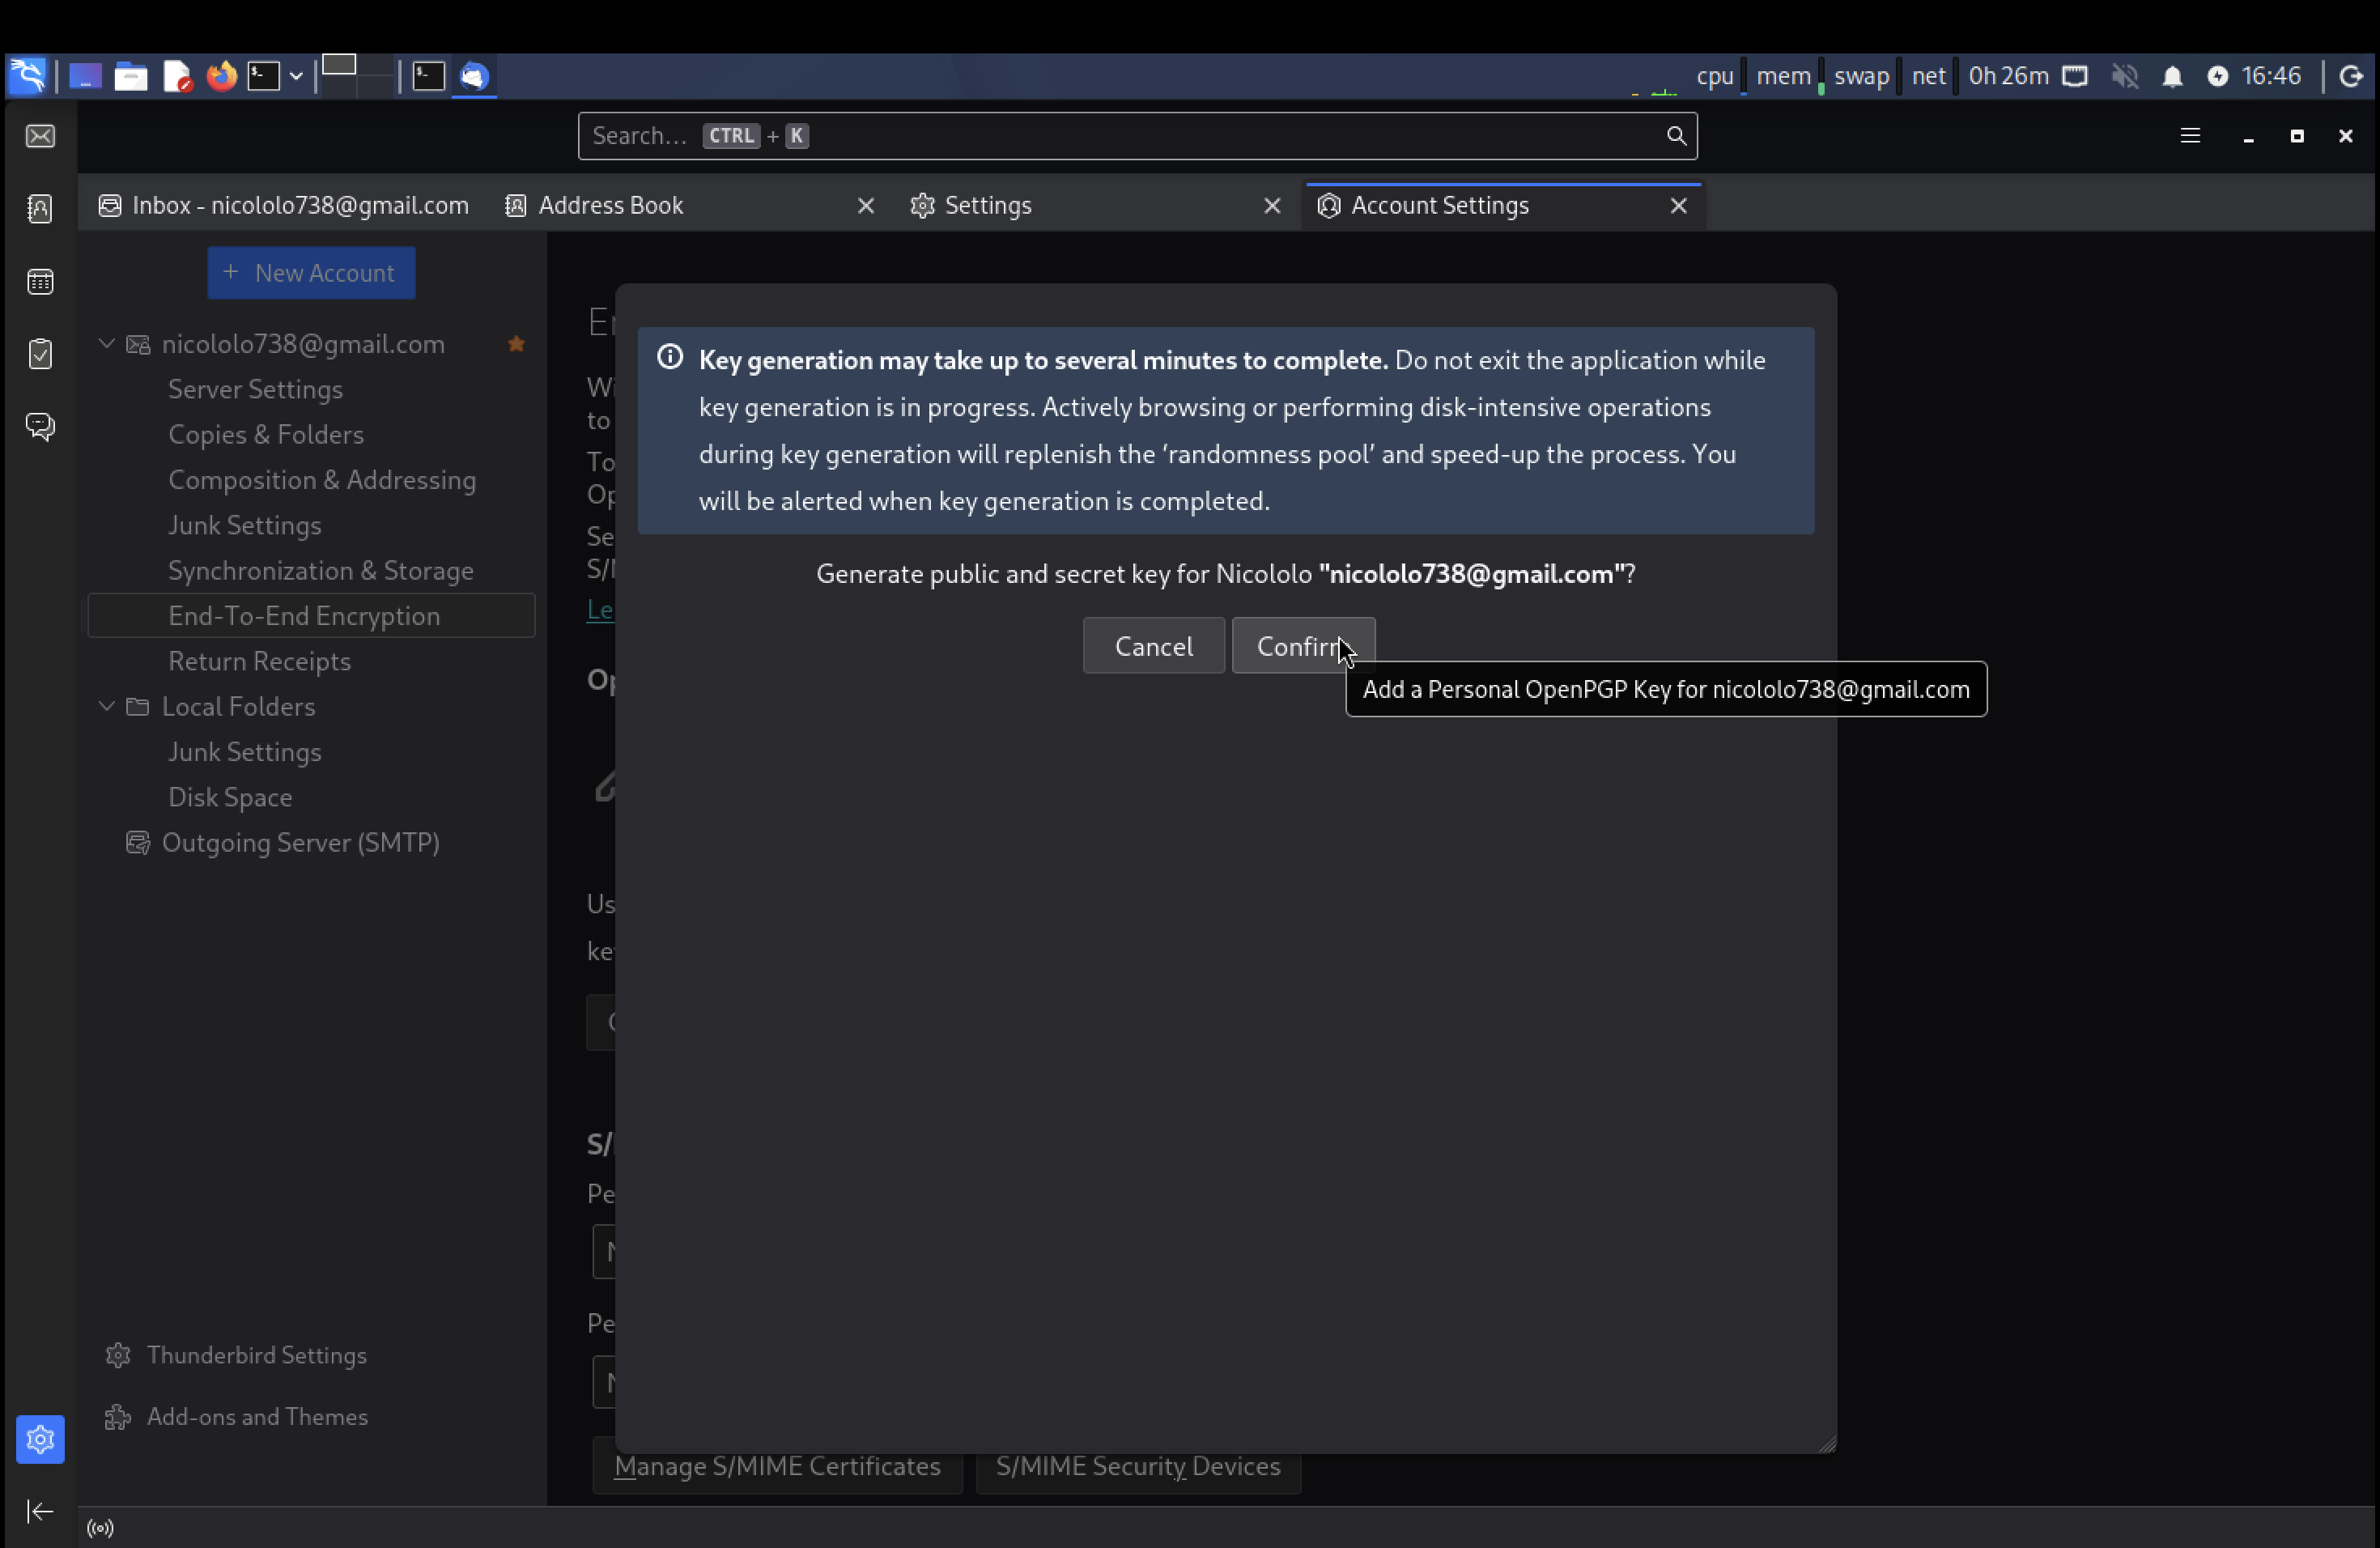
\includegraphics[width=0.85\textwidth]{Imagenes/4-CreationOfOpenPGPkey3.png}
    \caption{Diálogo de confirmación previo a la generación de la clave OpenPGP}
    \label{fig:confirmar_generacion}
\end{figure}

Una vez finalizado el proceso, la sección \textit{End-To-End Encryption} muestra la nueva clave asociada a la cuenta.

\section{Resumen de claves generadas}

\begin{table}[H]
    \centering
    \caption{Par de claves OpenPGP generado}
    \begin{tabularx}{\textwidth}{l|l}
        \toprule
        \textbf{Componente} & \textbf{Uso} \\
        \midrule
        Clave maestra & Firma (S) y Certificación (C) \\
        Subclave & Cifrado (E) \\
        \bottomrule
    \end{tabularx}
\end{table}

El par de claves queda almacenado en el llavero interno de Thunderbird y puede gestionarse desde \textbf{OpenPGP Key Manager} (accesible desde la barra de herramientas de composición).
